% http://www.ctan.org/tex-archive/macros/latex/contrib/beamer/examples
% http://latex.artikel-namsu.de/english/beamer-examples.html

%\documentclass{beamer}
\documentclass[usenames,dvipsnames]{beamer}
\usepackage{amsmath}
\usepackage{amssymb}
\usepackage{bm}
\usepackage{fancybox, graphicx}
\usepackage{listings}
\usepackage{tikz} % Diagrams
\usetikzlibrary{positioning}
\usepackage{color}
\usepackage{xcolor}
\usepackage{textcomp} % See https://tex.stackexchange.com/questions/145416/how-to-have-straight-single-quotes-in-lstlistings
%\usepackage[font=small,labelfont=bf]{caption} % Required for specifying captions to tables and figures. From https://tex.stackexchange.com/questions/238636
\usepackage[absolute,overlay]{textpos}




\usetheme{boxes}
\usecolortheme{beaver}


\title{MAF: \\ Masked Autoregressive Flow for Density Estimation}
\author{Lorne Whiteway \\ lorne.whiteway@star.ucl.ac.uk}
\institute{Astrophysics Group \\ Department of Physics and Astronomy \\ University College London}
\date{27 April 2020 \\ Find the presentation at \alert{\url{https://tinyurl.com/???}}}

\begin{document}

\frame{\titlepage}

\begin{frame}{Context}
  \begin{block}{}
    \begin{itemize}
      \item{\textit{Supervised machine learning} i.e. selecting from a highly-parameterised family of non-linear functions to fit some training data.}
      \item{Fitting is done to optimise a utility function that \textcolor{red}{rewards a close match to the training data} and \textcolor{blue}{penalises complexity i.e. enforces \textit{regularization}}.}
      \item{\textcolor{blue}{Regularisation is also provided by any lack-of-flexibility in the fitting functions.}}
      \item{Bayesian framework: \textcolor{red}{adherence to training data = likelihood}; \textcolor{blue}{regularisation = prior}.}
    \end{itemize}
  \end{block}
\end{frame}

\begin{frame}{Density Estimation}
  \begin{block}{}
    \begin{itemize}
      \item{We want to do ML to do density estimation:}
      \item{Find the probability density $p$, given a set of training data $\{x_i\}$ that we suppose to be a fair random sample from $p$.}
    \end{itemize}
  \end{block}
\end{frame}

\begin{frame}{MAF}
  \begin{block}{}
    \begin{itemize}
      \item{We will discuss the MAF algorithm: Papamakarios et al. 2018; Masked Autoregressive Flow for Density Estimation; \url{https://arxiv.org/abs/1705.07057}.}
      \item{Based on earlier algorithms of which the most relevant is MADE: Germain et al. 2015; MADE: Masked Autoencoder for Distribution Estimation; \url{https://arxiv.org/abs/1502.03509}.}
	\item{I will focus first on MADE as all the key ideas are present there.}
    \end{itemize}
  \end{block}
\end{frame}

\begin{frame}{Analogy}
  \begin{block}{}
    \begin{itemize}
      \item{An \textit{autoencoder} is like a parrot - it learns to mimic.}
	\item{An \textit{autoregressive autoencoder} is like a deaf parrot - it learns to play the probabilities (and hence becomes a density estimator).}
    \end{itemize}
  \end{block}
\end{frame}

\begin{frame}{Parrot training}
  \begin{block}{}
    \begin{itemize}
      \item{Simple example: single binary outcome. We want the parrot to mimic us when we say 'Yes' or 'No'.}
	\item{So give lots of 'Yes', 'No' training data; give the parrot treats but reduce the treats by the non-positive number $\log(\text{\% correctness of the parrot's response})$. This is called \textit{cross-entropy loss}.}
    \end{itemize}
  \end{block}
\end{frame}


\begin{frame}{Parrot training}
	\begin{columns}
           \column{0.58\linewidth}
    \begin{itemize}
      \item{The neural network is incentivised to model the identity function $\tilde{x_1} = x_1$.}
	\item{Depending on the flexibility of the neural network the parrot will get this exactly or approximately correct.}
    \end{itemize}
          \column{0.38\linewidth}
             \centering
             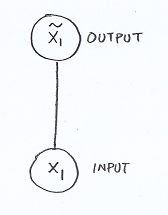
\includegraphics[height=5cm, width=3.5cm]{image_01}
         \end{columns} 
\end{frame}

\begin{frame}{Deaf parrot}
	\begin{columns}
           \column{0.58\linewidth}
    \begin{itemize}
      \item{Deaf parrot = no link between input and output.}
	\item{Parrot still squawks and gets feedback (more treats if the squawk accidentally matched the unheard training input).}
	\item{If say 75\% of the training data was 'Yes' then the parrot will learn to say 'Yes' more often. Optimal strategy will be a word that is 75\% 'Yes' and 25\% 'No'.}
    \end{itemize}
          \column{0.38\linewidth}
             \centering
             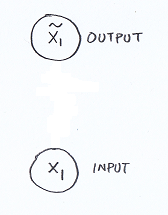
\includegraphics[height=5cm, width=3.5cm]{image_02}
         \end{columns} 
\end{frame}

\begin{frame}{Deaf parrot}
    \begin{itemize}
      \item{So by removing links from the neural network but still rewarding the network for mimicry we create a density estimator.}
    \end{itemize}
\end{frame}

\begin{frame}{Two word phrase}
    \begin{itemize}
      \item{Now consider two word phrases ("Yes, No").}
	\item{If there is no correlation between the two words then we just need two deaf parrots.}
	\item{But generally $p(x_1 \& x_2) = p(x_1) p(x_2 | x_1)$.}
	\item{To model this: one deaf parrot for $p(x_1)$ as before. But for the second parrot: unmask its ears, let it hear the training word told to the first parrot, the re-mask its ears for the second word.}
	\item{Give treats as before (still encouraging mimicry).}
	\item{Easy to show that the second parrot learns $p(x_2 | x_1)$.}
    \end{itemize}
\end{frame}


\begin{frame}{Two word phrase}
	\begin{columns}
           \column{0.46\linewidth}
    \begin{itemize}
    \item{More generally if $\tilde{x_i}$ is linked only to $x_1, \dots x_{i-1}$ then we learn $p(x_1), \dots, p(x_i | x1 \dots x_{i-1})$ whose product is $p(x)$.}
    \end{itemize}
          \column{0.5\linewidth}
             \centering
             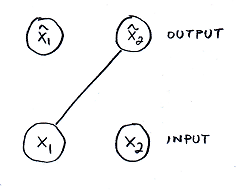
\includegraphics[height=5cm]{image_03}
         \end{columns} 
\end{frame}

\begin{frame}{Autoencoder; Autoregressive autoencoder}
    \begin{itemize}
      \item{The 'hearing' parrot (that mimics) is an \textit{autoencoder}.}
	\item{The network of partially-deaf parrots (that learns the conditional probabilities) is called an \textit{autoregressive autoencoder}.}
	\item{Autoregression appears in other contexts e.g. predicting the next element in a causal sequence.}
    \end{itemize}
\end{frame}

\begin{frame}{Figure 1 from MADE paper}
     \centering
     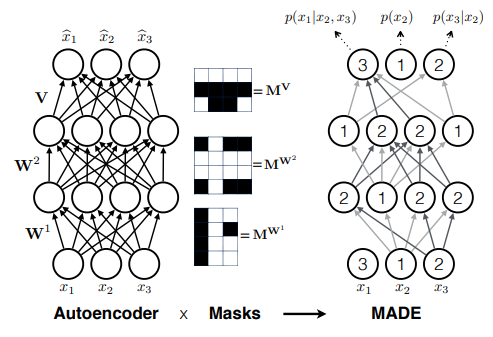
\includegraphics[height=7cm]{image_04}
\end{frame}

\begin{frame}{Sampling from the inferred probability density}
    \begin{itemize}
      \item{Use $(0, 0)$ as input to get $(\tilde{x_1}, \tilde{x_2})$ as output;}
	\item{Randomly choose $s_1$ in $\{0, 1\}$ with probability $\tilde{x_1}$ of being 1;}
	\item{Use $(s_1, 0)$ as input to get new $(\tilde{\tilde{x_1}}, \tilde{\tilde{x_2}})$ as output;}
	\item{Randomly choose $s_2$ in $\{0, 1\}$ with probability $\tilde{\tilde{x_2}}$ of being 1;}
	\item{Then $(s_1, s_2)$ is a new sample from the inferred density.}
	\item{Takes $D$ evaluations of the net to get one new sample.}
    \end{itemize}
\end{frame}


\begin{frame}{More complicated distributions}
    \begin{itemize}
      \item{So far we have looked at binary distributions.}
	\item{Here the probability density could be described by a single number ($= p(x_i = 1)$). So output $\tilde{x_i}$ has dual meaning as `best guess at $x_i$' and as `$p(x_i = 1 | x1, \dots, x_{i-1})$'.}
    \end{itemize}
\end{frame}

\begin{frame}{More complicated distributions}
    \begin{itemize}
      \item{To handle continuous distributions:}
	\item{Assume each univariate conditional distribution $p(x_i | x_1, \dots, x_{i-1})$ is Gaussian;}
	\item{Two output cells for each input: one for mean and one for (log of) standard deviation - from this we easily calculate the conditional probabilities and hence the overall probability of any given input;}
	\item{Loss function is now sum of negative logs of probabilities of training data.}
    \end{itemize}
\end{frame}


\begin{frame}{More complicated distributions}
     \centering
     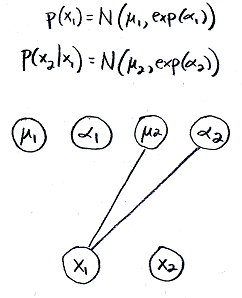
\includegraphics[height=7cm]{image_05}
\end{frame}


\begin{frame}{Sampling from the inferred probability density $\tilde{p}$}
    \begin{itemize}
      \item{As before we can create new samples with $D$ calls to the neural net.}
	\item{At each step we randomly choose $u_i$ from $N(0, 1)$ and scale and shift it to get $\tilde{x_i} = \exp(\alpha) * u_i + \mu$.}
	\item{At each step the $\alpha$ and $\mu$ come from a call to the net with $\tilde{x_1}, \dots, \tilde{x_{i-1}}$ as inputs.}
    \end{itemize}
\end{frame}

\begin{frame}{Sampling from the inferred probability density 1}
    \begin{itemize}
      \item{Thus we get a mapping $f$ from $u \sim N(0, I)$ to $\tilde{x} \sim \tilde{p}$.}
	\item{The mapping is easily invertible!}
	\item{$u_i = (\tilde{x_i} - \mu) \exp(-\alpha)$}
	\item{All the $\mu$ and $\alpha$ that we need are available in \textbf{one} call to the net (as here we have all the net input values that we need).}
	\item{This gives $f^{-1}$ mapping $\tilde{p}$ to $N(0, I)$.}
    \end{itemize}
\end{frame}

\begin{frame}{Sampling from the inferred probability density 2}
    \begin{itemize}
      \item{Furthermore the autoregressive property means that the Jacobian of $f^-1$ is triangular.}
	\item{Its diagonal elements are just the $exp(-\alpha_i)$ factors.}
	\item{So the determinant of $Jac(f^-1)$ is easy to calculate.}
    \end{itemize}
\end{frame}

\begin{frame}{Normalising flow}
    \begin{itemize}
      \item{So $f$ maps $N(0, I)$ to $\tilde{p}$.}
	\item{Such $f$ is called a normalising flow.}
	\item{Recall how probability densities transform: \\
	$\tilde{p}(x) = \mathcal{N}_{(0, I)}(f^{-1}(x)) \lvert det(Jac(f^{-1})) \rvert$}
	\item{All of these components are easy to calculate, and let us evaluate and sample from $\tilde{p}$.}
    \end{itemize}
\end{frame}

\begin{frame}{Example}
     \centering
     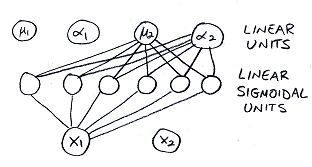
\includegraphics[height=5cm]{image_06}
\end{frame}



\end{document}
